In this section, a program to train a feedforward neural network with one hidden layer is described using pseudocode. It learns how to recognize handwritten digits from the MNIST database applying a stochastic gradient descent algorithm. Before starting with the rundown through the code, it is necessary a few key points are described pertaining  .

\section{Data structure}\label{DataStruct}
 The diagram below provides an overview of the main program divided in sections, to facilitate a quick and general understanding of the purpose of the functions and algorithms used in the project.\\
 
%begin{comment}
%:Title: Work breakdown structures aka WBS diagrams
%:Tags: Charts;Diagrams;Trees
%:Author: Gonzalo Medina
%:Slug: work-breakdown-structure

%A work breakdown structure (WBS) diagram, is for decomposing a task into smaller parts, which helps organizing and performing. This example diagram shows possible tasks for designing a TikZ diagram. The basis is a tree, nodes were addes below its child nodes. It was originally posted by Gonzalo Medina as TeX.SE (http://tex.stackexchange.com/q/81809/213), modified by Stefan Kottwitz.
%\end{comment}
\usetikzlibrary{arrows,shapes,positioning,shadows,trees}

\tikzset{
  basic/.style  = {draw, text width=3cm, drop shadow, font=\sffamily, rectangle},
  root/.style   = {basic, rounded corners=2pt, thin, align=center,
                   fill=blue!30},
  level 2/.style = {basic, rounded corners=6pt, thin,align=center, fill=gray!30,
                   text width=8em},
  level 3/.style = {basic, thin, align=left, fill=brown!60, text width=6.5em, scale = 0.9}
}

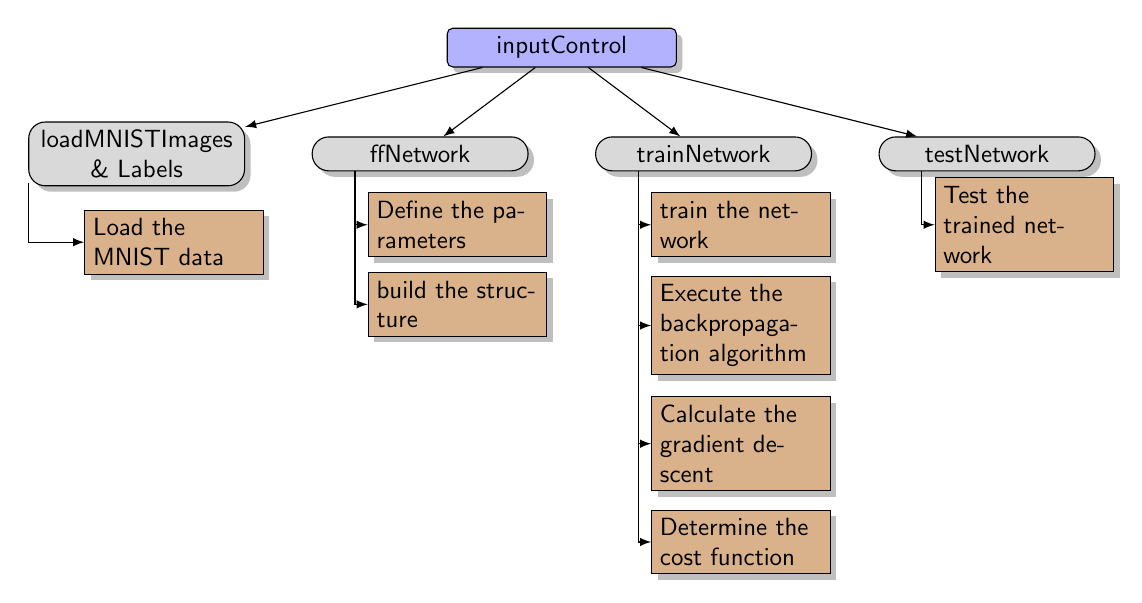
\begin{tikzpicture}[
  level 1/.style={sibling distance=40mm},
  edge from parent/.style={->,draw},
  >=latex,
  scale= 0.9
  ,every node/.style={scale= 0.9}]

% root of the the initial tree, level 1
\node[root] {inputControl}
% The first level, as children of the initial tree
  child {node[level 2] (c1) {loadMNISTImages \& Labels}}
  child {node[level 2] (c2) {ffNetwork}}
  child {node[level 2] (c3) {trainNetwork}}
  child {node[level 2] (c4) {testNetwork}};

% The second level, relatively positioned nodes
\begin{scope}[every node/.style={level 3}]
\node [below of = c1, xshift=15pt, yshift = - 7pt] (c11) {Load the MNIST data};

\node [below of = c2, xshift=15pt] (c21) {Define the parameters};
\node [below of = c21, yshift = -3.5pt] (c22) {build the structure};

\node [below of = c3, xshift=15pt] (c31) {train the network};
\node [below of = c31, yshift = -12pt] (c32) {Execute the backpropagation algorithm};
\node [below of = c32, yshift = -19pt] (c33) {Calculate the gradient descent};
\node [below of = c33, yshift = -11pt] (c34) {Determine the cost function};


\node [below of = c4, xshift=15pt] (c41) {Test the trained network};

\end{scope}

% lines from each level 1 node to every one of its "children"
\foreach \value in {1}
  \draw[->] (c1.195) |- (c1\value.west);

\foreach \value in {1,2}
  \draw[->] (c2.195) |- (c2\value.west);

\foreach \value in {1,2,3,4}
  \draw[->] (c3.195) |- (c3\value.west);
  
\foreach \value in {1}
  \draw[->] (c4.195) |- (c4\value.west);
  
  
  
\end{tikzpicture}\\
 
 In \textit{inputControl} you can set the parameters i.e. the number of minibatches, the number of neurons of each layer and the number of hidden layers. Included are four main functions \textit{loadMNISTImages}, \textit{Labels}, \textit{ffNetwork}, \textit{ trainNetwork} and the \textit{testNetwork}. The diagram describes the content of the functions. The structure of the program is clear and straight forward.\\
 
 Another important aspect when writing the code to train a network, is to decide how the data is going to be managed and stored. Generally, the programming language has some influence on the decision, due to the fact that different programs work on distinct programming bases. It is good practice to use matrices when programming in MATLAB, nevertheless, in our case we use cell arrays to store the weights and biases of the system, due to a versatile feature they possess: information can be stored in cell arrays regardless of data type and size. These can afterwards be listed in a structure array for clarity's sake. Using structures enables us to store any type of data in containers called fields, that way all the information can be grouped in one single variable, while allowing an easy access to single small groups of information. However, a few issues remain, for instance, cell arrays require more processing time than matrices.\\
 Considering the problem in question and given the relative simplicity of our neural network, we reached a compromise between an organized easy-to-follow structure over fast computing. Therefore, the numerical data for each layer is stored in cell arrays and these, in a structure array, e.g.:
 
 \includegraphics[scale=0.8]{Bilder/structArray.png}
 
 \includegraphics[scale=0.8]{Bilder/weightsMat.png}

\section{Algorithms}\label{Algorithms}

In this section we will present the main algorithms used to train the neural network as well as to test its performance and functioning. The description follows in pseudocode form.\\
\rule{\textwidth}{0.4pt}
 FEEDFORWARD: Returns the cell arrays "unactivatedOutput" and "activatedOutput" with the weighted inputs and activation values for each layer of the network after applying the feedforward algorithm iteratively. Returns a 1 if the input was correctly classified or a 0 if incorrectly in "classifiedCorrect".\\
\rule{\textwidth}{0.4pt}
\begin{addmargin}[2em]{0em}
\textbf{function} evaluate( \textbf{struct} modelParams, \textbf{double} data, dataLabel )\\
    $- \qquad$ \textbf{local variables:} int x[length(modelParams.model.hidden)]\\
    $- \qquad$ activatedOutput$_{input}$ $\leftarrow$ data\\
    $- \qquad $\\
    $- \quad $ \textit{Forward feeding}\\
    $- \qquad $ \textbf{for all} k = 2,3,...,x-1 \textbf{do}\\
    $- \qquad \quad $ unactivatedOutput $_k$ 
    $\leftarrow$ activatedOutput $_{k}*$ weights$_{k}$ - biases$_{k}$ \\
    $- \qquad \quad $ activatedOutput $_{k+1}$ 
    $\leftarrow$ activate(unactivatedOutput $_k$)\\
    $- \qquad $ \textbf{end for}\\
    $- \qquad $\\
    $- \quad $ \textit{Control}\\
    $- \qquad $ \textbf{if} activatedOutput $_{output}$ $\Longleftrightarrow$ dataLabel\\
    $- \qquad \quad$ classifiedCorrect $\leftarrow$ 1\\
    $- \qquad$ \textbf{end if}\\
    $- \qquad$ \textbf{return} classifiedCorrect, activatedOutput,  unactivatedOutput\\
\textbf{end function}\\
\end{addmargin}
\rule{\textwidth}{0.4pt}
 BACKPROPAGATION: Returns the cell arrays "deltaGradWeights" and "deltaGradBiases" with the gradient of the cost function for the weights and the biases respectively calculated with the backpropagation algorithm.\\
\rule{\textwidth}{0.4pt}
\begin{addmargin}[2em]{0em}
\textbf{function} backprop( \textbf{struct} modelParams, \textbf{double} data, dataLabel )\\
    $- \qquad$ \textbf{local variables:} int x[length(modelParams.model.hidden)+2]\\
    $- \qquad$ unactivatedOutput, activatedOutput $\leftarrow$ evaluate(modelParams, data)\\
    $- \qquad $\\
    $- \quad $ \textit{Propagating the gradient bacwards starting at output layer}\\
    $- \qquad$ deltaGradBiases$_{output}$ $\leftarrow$ deriveCost(dataLabel, activatedOutput${_x}$)\\
    $- \qquad$ deltaGradWeights$_{output}$ $\leftarrow$ activatedOutput$_{x-1}*$ deltaGradBiases$_{output}$\\
    $- \qquad $ \textbf{for all} k = 2,3,...,x-1 \textbf{do}\\
    $- \qquad \quad $ deltaGradBiases $_{x-k}$ 
    $\leftarrow$ deltaGradBiases$_{x-k+1}*$modelParams.weights$_{x-k+1}$\\
    $- \qquad \quad $ deltaGradWeights $_{x-k}$ 
    $\leftarrow$ activatedOutput$_{x-k}*$ deltaGradBiases$_{x-k}$\\
    $- \qquad $ \textbf{end for}\\
    $- \qquad$ \textbf{return} deltaGradWeights, deltaGradBiases\\
\textbf{end function}\\
\end{addmargin}
\rule{\textwidth}{0.4pt}
 ADJUSTING PARAMETERS: Returns the updated structure array "modelParams" after applying the backpropagation algorithm on each input of a single batch.\\
\rule{\textwidth}{0.4pt}
\begin{addmargin}[2em]{0em}
\textbf{function} adjustParams( \textbf{struct} modelParams, \textbf{double} data, dataLabel )\\
    $- \qquad$ \textbf{local variables:} int x[length(data)]\\
    $- \qquad $ \textbf{for all} k = 1,2,...,x \textbf{do}\\
    $- \qquad \quad$ deltaGradWeights, deltaGradBiases $\leftarrow$\\
    $- \qquad \qquad \quad \qquad $ backprop(modelParams, data$_{k}$  , dataLabel$_{k}$)\\
    $- \qquad $\\
    $- \qquad $ \textit{Updating weights and biases}\\
    $- \qquad \quad$ \textbf{local variables:} int y[length(deltaGradWeights)]\\
    $- \qquad \quad $ \textbf{for all} l = 1,2,...,y \textbf{do}\\
    $- \qquad \quad \quad$ modelParams.weights$_{l}$ $\leftarrow$ modelParams.weights$_{l}$ - eta/x $*$deltaGradWeights$_{l}$\\
    $- \qquad \quad \quad$ modelParams.biases$_{l}$ $\leftarrow$ modelParams.biases$_{l}$ - eta/x $*$deltaGradBiases$_{l}$\\
    $- \qquad \quad$ \textbf{end for}\\
    $- \qquad$ \textbf{end for}\\
    $- \qquad$ \textbf{return} modelParams\\
\textbf{end function}\\
\end{addmargin}
\rule{\textwidth}{0.4pt}
 TRAINING: Returns the structure array "modelParams" with the network's final parameters after training it using stochastic gradient descent with two stopping criteria: "accuracy" and maximum number of iterations. Returns the vector "cost" with the value of the cost function after every iteration and the value "epoch" with the total number of iterations.\\
\rule{\textwidth}{0.4pt}
\begin{addmargin}[2em]{0em}
\textbf{function} trainNetwork( \textbf{struct} model, \textbf{double} data, dataLabel )\\
    $- \qquad$ \textbf{local variables:} int epoch, x[length(data(:,1))], y[batchSize]\\
    $- \qquad $ \textbf{while} model.averageCostChange $>$ accuracy \textbf{AND} epoch$<$100 \textbf{do}\\
    $- \qquad \quad$ epoch $\leftarrow$ epoch + 1\\
    $- \qquad $\\
    $- \qquad $ \textit{Learning}\\
    $- \qquad \quad$ \textbf{for all} k = 1,2,...,x/y \textbf{do}\\
    $- \qquad \quad \quad  $ modelParams $\leftarrow$ adjustParams(modelParams,data$_k$, dataLabel$_k$) \\ 
    $- \qquad \quad $ \textbf{end for}\\
    $- \qquad $\\
    $- \qquad $ \textit{Calculating cost of an iteration}\\
    $- \qquad \quad $ cost $_{epoch}$
    $\leftarrow$ calcCost(modelParams, data, dataLabel)\\
    $- \qquad \quad$ \textbf{if} mod(epoch, model.averageOverEpochs) == 0\\
    $- \qquad \quad \quad$ \textbf{for all} k = 1,2,...,model.averageOverEpochs - 1 \textbf{do}\\
    $- \qquad \quad \quad \quad $costChange $\leftarrow$ cost$_{epoch-k+1}$ - cost$_{epoch-k}$\\
    $- \qquad \quad \quad$ \textbf{end for}\\
    $- \qquad \quad$ model.averageCostChange $\leftarrow$\\
    $- \qquad \quad \quad \quad \quad$ abs(sum(costChange)/(model.averageOverEpochs - 1))\\
    $- \qquad \quad$ \textbf{end if}\\
    $- \qquad$ \textbf{end while}\\
    $- \qquad$ \textbf{return} modelParams, cost, epoch\\
\textbf{end function}\\
\end{addmargin}
\rule{\textwidth}{0.4pt}
 TESTING: Returns the value of the ratio of correctly identified inputs over total number of inputs.\\
\rule{\textwidth}{0.4pt}
\begin{addmargin}[2em]{0em}
\textbf{function} testNetwork( \textbf{struct} modelParams, \textbf{double} data, dataLabel )\\
    $- \qquad$ \textbf{local variables:} int x[length(data(:,1))]\\
    $- \qquad $\\
    $- \quad $ \textit{Forward feeding to get output on test-set with trained network}\\
    $- \qquad $ \textbf{for all} k = 1,2,...,x \textbf{do}\\
    $- \qquad \quad $ results$_k$ $\leftarrow$ evaluate( modelParams,  data$_{k}$, dataLabel$_{k}$)\\
    $- \qquad $ \textbf{end for}\\
    $- \qquad $\\
    $- \quad $ \textit{Computing accuracy}\\
    $- \qquad $ modelResult $\leftarrow$ sum(results)/(length(results))\\
    $- \qquad$ \textbf{return} modelResult\\
\textbf{end function}\\
\end{addmargin}

The pseudocode below shows the way to run the code and get the sought-after information:\\
\rule{\textwidth}{0.4pt}
\textbf{inputControl:} TRAINING AND TESTING A FF-NEURAL NETWORK\\
\rule{\textwidth}{0.4pt}
\rule{\textwidth}{0.4pt}
NETWORK'S CHARACTERISTICS AND HYPER-PARAMETERS: Defining the learning rate "eta", the size of the batches in which the data-set is divided for the SGD "batchSize", and the activation function and its derivative in the object "activationFunction" of the class "activation".\\
\rule{\textwidth}{0.4pt}
\rule{\textwidth}{0.4pt}
\begin{addmargin}[2em]{0em}
\textbf{global variables:} \\
$- \qquad$ \textbf{double} eta\\
$- \qquad$ \textbf{double} batchSize\\
$- \qquad$ \textbf{activation} activationFunction (@sig, @sigDerivative)\\
$-$\\
\textbf{Loading MNIST data}\\
$- \qquad$ testData $\leftarrow$ loadMNISTImages('path to testing images')\\
$- \qquad$ testLabel $\leftarrow$ loadMNISTLabels('path to testing images' labels')\\
$- \qquad$ trainData $\leftarrow$ loadMNISTImages('path to training images')\\
$- \qquad$ trainLabel $\leftarrow$ loadMNISTLabels('path to training images' labels')\\
$-$\\
\textbf{Network's configuration}\\
$- \qquad$ model $\leftarrow$ ffNetwork(activationFunction, eta, batchSize, 784, 10, 30)\\
$-$\\
\textbf{Procedure:} TRAINING\\
$- \qquad$ modelParams, cost, epoch $\leftarrow$ trainNetwork(model, trainData, \\
$- \qquad \qquad  $trainLabel)\\
$-$\\
\textbf{Procedure:} TESTING\\
$- \qquad$ modelResult $\leftarrow$ testNetwork(modelParams, testData, testLabel)\\
\end{addmargin}

\section{Functions}\label{Functions}

In this section each of the functions utilized by the training and testing algorithms are listed.\\
\rule{\textwidth}{0.4pt}
PARSING DATA: Returns matrix "images" of size (number of images X 784 pixels) with the images and column vector "labels" of size (number of labels X 1) with the labels for each image from the MNIST data-set.\\
\rule{\textwidth}{0.4pt}
\begin{addmargin}[2em]{0em}
\textbf{function} loadMNISTImages(\textbf{string} path to images)\\
    $- \qquad$fp $\leftarrow$ open path to images\\
    $- \qquad$images $\leftarrow$ read fp\\
    $- \qquad$ \textbf{return} images\\
\textbf{end function}\\
\end{addmargin}
\begin{addmargin}[2em]{0em}
\textbf{function} loadMNISTLabels(\textbf{string} path to labels)\\
$- \qquad$ fp $\leftarrow$ open path to labels\\
    $- \qquad$ labels $\leftarrow$ read fp\\
    $- \qquad$ \textbf{return} labels\\
\textbf{end function}\\
\end{addmargin}
\rule{\textwidth}{0.4pt}
ACTIVATION: Defines a class "activation". The objects from this class have the methods "activate" and "deriveActivation" which computes the activation function on an input and its derivative respectively.\\
\rule{\textwidth}{0.4pt}
\begin{addmargin}[2em]{0em}
\textbf{class} activation\\
    $- \qquad$\textbf{properties}\\
    $- \qquad \quad$ activate\\
    $- \qquad \quad$ deriveActivation\\
    $- \qquad$ \textbf{end properties}\\
    $- \qquad$ \textbf{methods}\\
    $- \qquad \quad$ \textbf{function} activation(Function, Derivative)\\
    $- \qquad \quad \quad $obj.activate $\leftarrow$ Function\\
    $- \qquad \quad \quad $obj.deriveActivation $\leftarrow$ Derivative\\
    $- \qquad \quad$ \textbf{end function}\\
    $- \qquad$ \textbf{end methods}\\
\textbf{end class}\\
\end{addmargin}
\rule{\textwidth}{0.4pt}
SIGMOID FUNCTION: Returns the vector "result" with the calculated sigmoid function of an input "x".\\
\rule{\textwidth}{0.4pt}
\begin{addmargin}[2em]{0em}
\textbf{function} sig( \textbf{double} x )\\
    $- \qquad$ result $\leftarrow$ sigmoid function x \\
    $- \qquad$ \textbf{return} result\\
\textbf{end function}\\
\end{addmargin}
\rule{\textwidth}{0.4pt}
DERIVATIVE SIGMOID FUNCTION: Returns the vector "result" with the calculated derivative of a sigmoid function of an input "x".\\
\rule{\textwidth}{0.4pt}
\begin{addmargin}[2em]{0em}
\textbf{function} sigDerivativ( \textbf{double} x )\\
    $- \qquad$ result $\leftarrow$ sigmoid function derivative x \\
    $- \qquad$ \textbf{return} result\\
\textbf{end function}\\
\end{addmargin}
\rule{\textwidth}{0.4pt}
DERIVATIVECOST FUNCTION: Returns the vector "dC" with the calculated derivative of the cost function of an input "actualOutput" and the desired value to the input "desiredOutput".\\
\rule{\textwidth}{0.4pt}
\begin{addmargin}[2em]{0em}
\textbf{function} deriveCost( \textbf{double} desiredOutput, actualOutput)\\
    $- \qquad$ dC $\leftarrow$ actualOutput - desiredOutput \\
    $- \qquad$ \textbf{return} desiredOutput, actualOutput\\
\textbf{end function}\\
\end{addmargin}
\rule{\textwidth}{0.4pt}
CONFIGURING NETWORK: Returns the structure array "model" loaded with all necessary parameters to create the initial network.\\
\rule{\textwidth}{0.4pt}
\begin{addmargin}[2em]{0em}
\textbf{function} ffNetwork( \textbf{activation} af, \textbf{double} eta, batchsize, in, hid, out )\\
    $- \qquad$ model $\leftarrow$ af, eta, batchsize, in, hid, out \\
    $- \qquad$ \textbf{return} model\\
\textbf{end function}\\
\end{addmargin}
\rule{\textwidth}{0.4pt}
INITIALIZING NETWORK: Returns the cell arrays "weights" and "biases" with the randomly generated weights and biases for each layer of the initial network.\\
\rule{\textwidth}{0.4pt}
\begin{addmargin}[2em]{0em}
\textbf{function} ffNetwork( \textbf{struct} model )\\
    $- \qquad$ \textbf{local variables:} int x[length(model.hidden)]\\
    $- \qquad$ weights$_{input}$, biases$_{input}$ $\leftarrow$ randn(model.input)\\
    $- \qquad$ \textbf{if} x $>$ 1\\
    $- \qquad \quad $ \textbf{for all} k = 2,3,...,x \textbf{do}\\
    $- \qquad \qquad \quad $ weights$_k$ $\leftarrow$ randn(model.hidden(k-1),model.hidden(k))\\
    $- \qquad \qquad \quad $ biases$_k$$\leftarrow$ randn(model.hidden(k))\\
    $- \qquad \quad $ \textbf{end for}\\
    $- \qquad $ \textbf{end if}\\
    $- \qquad$ weights$_{output}$, biases$_{output}$ $\leftarrow$ randn(model.output)\\
    $- \qquad$ \textbf{return} weights, biases\\
\textbf{end function}\\
\end{addmargin}
\rule{\textwidth}{0.4pt}
 CALCULATE COST: Returns the value of the cost function for a set of inputs "data" and corresponding expected outputs "labels".\\
\rule{\textwidth}{0.4pt}
\begin{addmargin}[2em]{0em}
\textbf{function} calcCost( \textbf{struct} modelParams, \textbf{double} data, dataLabel )\\
    $- \qquad$ \textbf{local variables:} int x[size(data,1)], double costVec, labelsVec\\
    $- \qquad $ \textbf{for all} k = 2,3,...,x \textbf{do}\\
    $- \qquad \quad $ labelsVec(dataLabel$_k$ + 1)$\leftarrow$ 1 \\ 
    $- \qquad \quad $ activatedOutput $\leftarrow$ evaluate( modelParams,  data$_{k}$, dataLabel$_{k}$)\\
    $- \qquad \quad $ costVec $_{k}$
    $\leftarrow$ norm(labelsVec - activatedOutput)$^2$\\
    $- \qquad \quad $ labelsVec(dataLabel$_k$ + 1)$\leftarrow$ 0 \\ 
    $- \qquad $ \textbf{end for}\\
    $- \qquad $ cost $\leftarrow$ sum(costVec)/(2 $*$ x)\\
    $- \qquad$ \textbf{return} cost\\
\textbf{end function}\\
\end{addmargin}

\section{Testing}
\subsection{Test: decrease of cost function}
To test our implementation, specifically to verify that the learning works as expected, we evaluated the cost function along the training process and checked if it actually decreased. Figure \ref{fig:costTrainSet} shows two cost curves for the same parameter bundle (detailed parameters in the image caption) but different learning rates evaluated on the training set. In both cases it can be clearly seen that the cost is decreasing after each epoch and thereafter saturates at a level close to zero. While for a learning rate of eta = 3 the cost curve has some bumps in it and even slightly increases from epoch 12 to 13, the cost curve with eta = 0.5 is much smoother but also takes more than twice as many epochs to reach a comparable cost level. 
\begin{figure}[t!]
\centering
    \begin{subfigure}[t]{0.49\textwidth}
        \centering
        \includegraphics[width=1.1\textwidth]{test_src/img/eta3_trainset}
        \caption{learning rate eta = 3.0}
    \end{subfigure}
    \begin{subfigure}[t]{0.49\textwidth}
        \centering
        \includegraphics[width=1.1\textwidth]{test_src/img/eta05_trainset}
        \caption{learning rate eta = 0.5}
    \end{subfigure}
    \caption{Cost function evaluated on the whole training set (60000 inputs) with a batch size of 10 and 30 neurons in the hidden layer. }
    \label{fig:costTrainSet}
\end{figure}

% (in the following referred as epoch curve)

\subsection{Test: the backpropagation algorithm}
The backpropagation algorithm in the \textit{backprop.m} file is used to calculate the gradient of the cost function in respect to all weights and biases. To check if the algorithm is implemented correctly, the same derivatives can be calculated in a numerical way using equation \eqref{eq:numDerivativ}, where $v$ is a random number and $\epsilon$ goes to zero.
\begin{align}
    f'(x) = \lim_{\epsilon \to 0} \frac{f(x + \epsilon \times v) - f(x - \epsilon \times v )}{2\epsilon}
    \label{eq:numDerivativ}
\end{align}
According to the equation above the difference of the numeric and the analytic derivatives $g(x)$ should approach zero as $\epsilon$ gets smaller. That is:
\begin{align}
f'(x) -v\times g(x) = \mathcal{O}(\epsilon)
    \label{eq:condition}
\end{align}
The matlab script \textit{backpropTest.m} uses equation \eqref{eq:condition} to ascertain the right implementation of the backpropagation algorithm. It uses an empirical value for the learning rate $\epsilon$ of $10^{-4}$ \footnote{\url{http://ufldl.stanford.edu/wiki/index.php/Gradient_checking_and_advanced_optimization}}, and corroborates condition \eqref{eq:condition} for each weight and bias of a network. It has shown that the difference is of the magnitude $\mathcal{O}(10^{-12})$, for all weights and biases, which can be taken as a proof that the backpropagation algorithm is correct.  